%%%%%%%%%%%%%%%%%%%%%%%%%%%%%%%%%%%%%%%%%%%%%%%%%%%%%%%%%%%%%%%%%%%%%%%%%%%%%%
% CONTRIBUTION TO THE MESONH BOOK1: "Bogusing for cyclones"
% Author: Olivier Nuissier
% Original : March 27, 2008
%%%%%%%%%%%%%%%%%%%%%%%%%%%%%%%%%%%%%%%%%%%%%%%%%%%%%%%%%%%%%%%%%%%%%%%%%%%%%%%

\chapter{Bogusing for Cyclones}

\minitoc
\section{Introduction}
Mature tropical cyclones are very intense atmospheric disturbances with 
typical horizontal extent of several hundred to a thousand kilometers, 
occurring over the most earth's tropical oceanic regions. Wind, storm surges 
and inland flooding generally associated with tropical cyclones cause, 
every year, losing of human lives and major material damages in many 
countries of the tropical belt. Dedicated airborne missions performed over 
the Atlantic using Doppler radars, but also generally coastal Doppler 
measurements can permit to deduce kinematic and thermodynamic structure of 
the vortex. 

Meanwhile, since early of 70's, tropical cyclone modeling significantly 
improved with using of sophisticated parameterization schemes of convection, 
microphysics, turbulence, surface fluxes,... However, one major drawback of many 
numerical studies of tropical cyclone is the fact that the initial vortex, 
usually obtained from global analyses, is often ill-defined, too weak, and 
sometimes misplaced, leading to subsequent simulation of storm track, structure, 
and intensity.

The following approach is the one proposed by Nuissier et al. (2005) is which 
airborne Doppler radar data are used to define a 'specified vortex' for Meso-NH
model initialization.

\section{Method}


\subsection{Removal of the analyzed vortex}

To incorporate a hurricane-like vortex with realistic size, depth, and intensity 
in the Meso-NH initial conditions, it is first necessary to remove the weak 
vortex analyzed by global models. For this purpose, the scheme proposed by 
Kurihara et al. (1993 (hereafter KBR93), 1995) is applied.
It consists of using appropriate numerical  filters to extract the vortex
from the large-scale analysis and adding a vortex specified from observations.
This can be written symbolically as:

\begin{equation}
[h_{i}]=[h]-[h_{av}]+[h_{s}]
\end{equation}

where [h$_{i}$] is the initial field, [h] is the global analysis, [h$_{av}$] is 
the analyzed vortex and [h$_{s}$] is the specified vortex.

A low-pass filter with an exponential weighting function is first applied to the 
modified large-scale analysis field [h] over the outermost Meso-NH domain to 
remove features with wavelengths smaller than about 1200 km, the characteristic 
dimension of the analyzed vortex. Using the same terminology as KBR93, this 
produces the basic field [h$_{b}$], which is subtracted from [h] to obtain the 
total disturbance field [h$_{d}$]:

\begin{equation}
[h]-[h_{b}]=[h_{d}]=[h_{av}]+[h_{nh}]
\label{hb}
\end{equation}

where [h$_{nh}$] is the none-hurricane disturbance.

The next step consists of extracting [h$_{av}$] from [h$_{d}$]. This is done 
using the same cylindrical filter as that proposed by KBR93:

\begin{equation}
h_{av}(r,\theta)=h_{d}(r,\theta)-[h_{d}(r_{0},\theta)E(r)+h_{d}(r_{0})(1-E(r))]
\end{equation}

where r and $\theta$ are the radius and the azimuth relative to the center  of the 
analyzed vortex, r$_{0}$ is the radius at which the value of weighting function 
E(r)=1, and h$_{d}$(r$_{0}$) is the mean value of h$_{d}$(r,$\theta$) for r=r$_{0}$ 
and 0 $\le$ $\theta$ $<$ 2$\pi$. The function E(r) (see Eq. (3.8) and Fig. 2(b) in 
KBR93) is an empirically determined exponential equation which increases smoothly 
from 0 at r=0 to 1 at r=r$_{0}$, with a smooth transition between the inner (i.e. 
hurricane component for r$<$r$_{0}$) and the outer regions (i.e. non-hurricane 
component for r$>$r$_{0}$).

\subsection{A 'specified vortex' derived from airborne Doppler radar observations}

After the analyzed vortex has been removed, the resulting environmental fields are 
used as new large-scale conditions, and interpolated over the other innermost Meso-NH 
domains. A symmetrical radar-derived vortex deduced from Doppler radar observations 
is then added to this modified large-scale field in every Meso-NH domains. This 
method is referred to as the 'Radar Vortex Conditioning' (RVC).

The wave number-0 component (symmetrical part) of the tangential wind is first 
deduced from the Extended Velocity-Track Display (EVTD) or Ground-Based 
Velocity-Track Display (GB-VTD) analysis (Roux and Marks 1996, Roux et al. 2004). Although the EVTD-derived velocities bring valuable information on the storm dynamic structure, they do not cover a large enough domain to properly define the specified vortex. Hence, an analytic model is used to describe the radial and vertical 
distribution of the tangential wind over a larger domain. The analytic wind 
V$_{T}$(r,z), where z is altitude, is defined through a simplified version of the 
formulation proposed by Holland (1980), as:

\begin{equation}
V_{T}(r,z)=V_{Tmax}(z) \left\langle \dfrac{exp\left\lbrace 1-1/\left[ r/RMW(z)\right]^{B(z)}\right\rbrace } {[r/RMW(z)]^{B(z)}} \right\rangle^{1/2} 
\label{VT(r,z)}
\end{equation}

where V$_{Tmax}$(z) is the maximum wind, RMW(z) is the radius of maximum wind, and 
B(z) is a scaling parameter for the radial variation of the wind. In order to avoid 
spurious variations of V$_{Tmax}$, RMW and B between the different levels, they 
suppose to obey the following relations with respect to z:

\begin{equation}
V_{Tmax}(z)=V_{Tmax_0} \left(\dfrac{1-z}{17.5 km} \right)^C 
\label{VTmax(z)}
\end{equation} 

\begin{equation}
RMW(z)=RMW_0+RMW_z \times z+RMW_{zz} \times z^2
\label{RMW(z)}
\end{equation}

\begin{equation}
B(z)=B_0+B_z \times z+B_{zz} \times z^2
\label{B(z)}
\end{equation}

where B$_{0}$, B$_{z}$, B$_{zz}$ are constants. Once V$_{Tmax}$(z) and RMW(z) have 
been determined at each level from the EVTD-derived tangential winds, coefficients 
V$_{Tmax_0}$  and C in (\ref{VTmax(z)}), RMW$_{0}$, RMW$_{z}$, RMW$_{zz}$ in (\ref{RMW(z)})
are deduced from least-squares fits along the vertical. Then, parameters B$_{0}$, B$_{z}$, B$_{zz}$ in (\ref{B(z)}) are deduced from a least-squares fit of the 
EVTD-derived winds in the radius-height domain, with the constraint that B(z) must be 
between 1.0 and 2.5 (Holland 1980).


\subsection{The thermal-wind balance}

As shown by other studies, a numerical model may produce more realistic tropical 
cyclones when a specified vortex includes wind and sea-level pressure information. 
Pressure perturbations associated with a tropical cyclone are mainly caused by 
hydrostatic effects due to the warm anomaly at its center. Hence, the specified 
vortex to be added to the large-scale analysis must include complementary descriptions 
of the cyclonic wind and temperature perturbations. Temperature can be deduced from 
the analytic tangential wind V$_{T}$(r,z) in (\ref{VT(r,z)}) through the thermal-wind 
relation:

\begin{equation}
\frac{\partial}{\partial r}\theta_{1}(r,z)=\frac{\theta_{0}(z)}{g}\left[2\frac{V_{T}(r,Z)}{r}+f\right]\frac{\partial}{\partial\zeta}V_{T}(r,Z) 
\label{tempe_pert}
\end{equation}

where $\theta_{0}$(z) is the potential temperature in the environment ([h$_{b}$] in 
\ref{hb}), $\theta_{1}$(r,z) is the cyclonic perturbation, f is the Coriolis parameter, g is the acceleration due to gravity, Z is a modified vertical coordinate 
such that Z = z $\times\left\langle\theta_{0}\right\rangle$ / $\theta_{0}$(z), where 
$\left\langle\theta_{0}\right\rangle$ is the mean value of $\theta_{0}$(z). $\theta_{1}(r,z)$ is obtained from the horizontal integration of (\ref{tempe_pert}) 
starting from 0 at 300 km radius. Of course due to the exponential decrease of the 
analytic tangential wind in (\ref{VT(r,z)}), it is not strictly correct to suppose that 
temperature perturbations vanish at 300 km radius. However, the relatively weak value 
of radial gradient of V$_{T}(r,z)$ beyond this limit makes the difference quite negligible.

It must be emphasized that the EVTD analysis could permit to retrieve a realistic structure of the secondary circulation (i.e. updraft centered on the radius of maximum wind, inflow (outflow) in the lower (upper) part of troposphere). In the 
numerical models (as in reality) the radial and vertical circulation results from: 
sensible- and latent-heat fluxes from the ocean surface increasing $\theta_{e}$ in 
the lowest atmospheric layers; surface friction inducing radial convergence; 
latent-heat release sustaining vertical motions through thermal buoyancy; and 
vertical momentum fluxes generating horizontal and vertical pressure perturbation 
gradients. Including these physical constraints in an analytical formulation of a 
symmetric secondary circulation would be a very difficult task. Therefore, only a balanced symmetric tangential circulation is added in the initial conditions 
of Meso-NH model for the moment.

Figure \ref{bogus} illustrates the RVC methodology for the case of Hurricane Bret on 22-23 August 1999 over the Gulf of Mexico, from the ECMWF large-scale analysis. Fig. \ref{bogus}a shows that the ECMWF model, because its coarse horizontal resolution, failed to properly reproduce the mature hurricane, whereas the 'specified' radar vortex highlights wind maximum intensity much stronger and closer to the hurricane center (Fig. \ref{bogus}b). 


\begin{figure}[!ht]
\centerline{\begin{tabular}{cc}
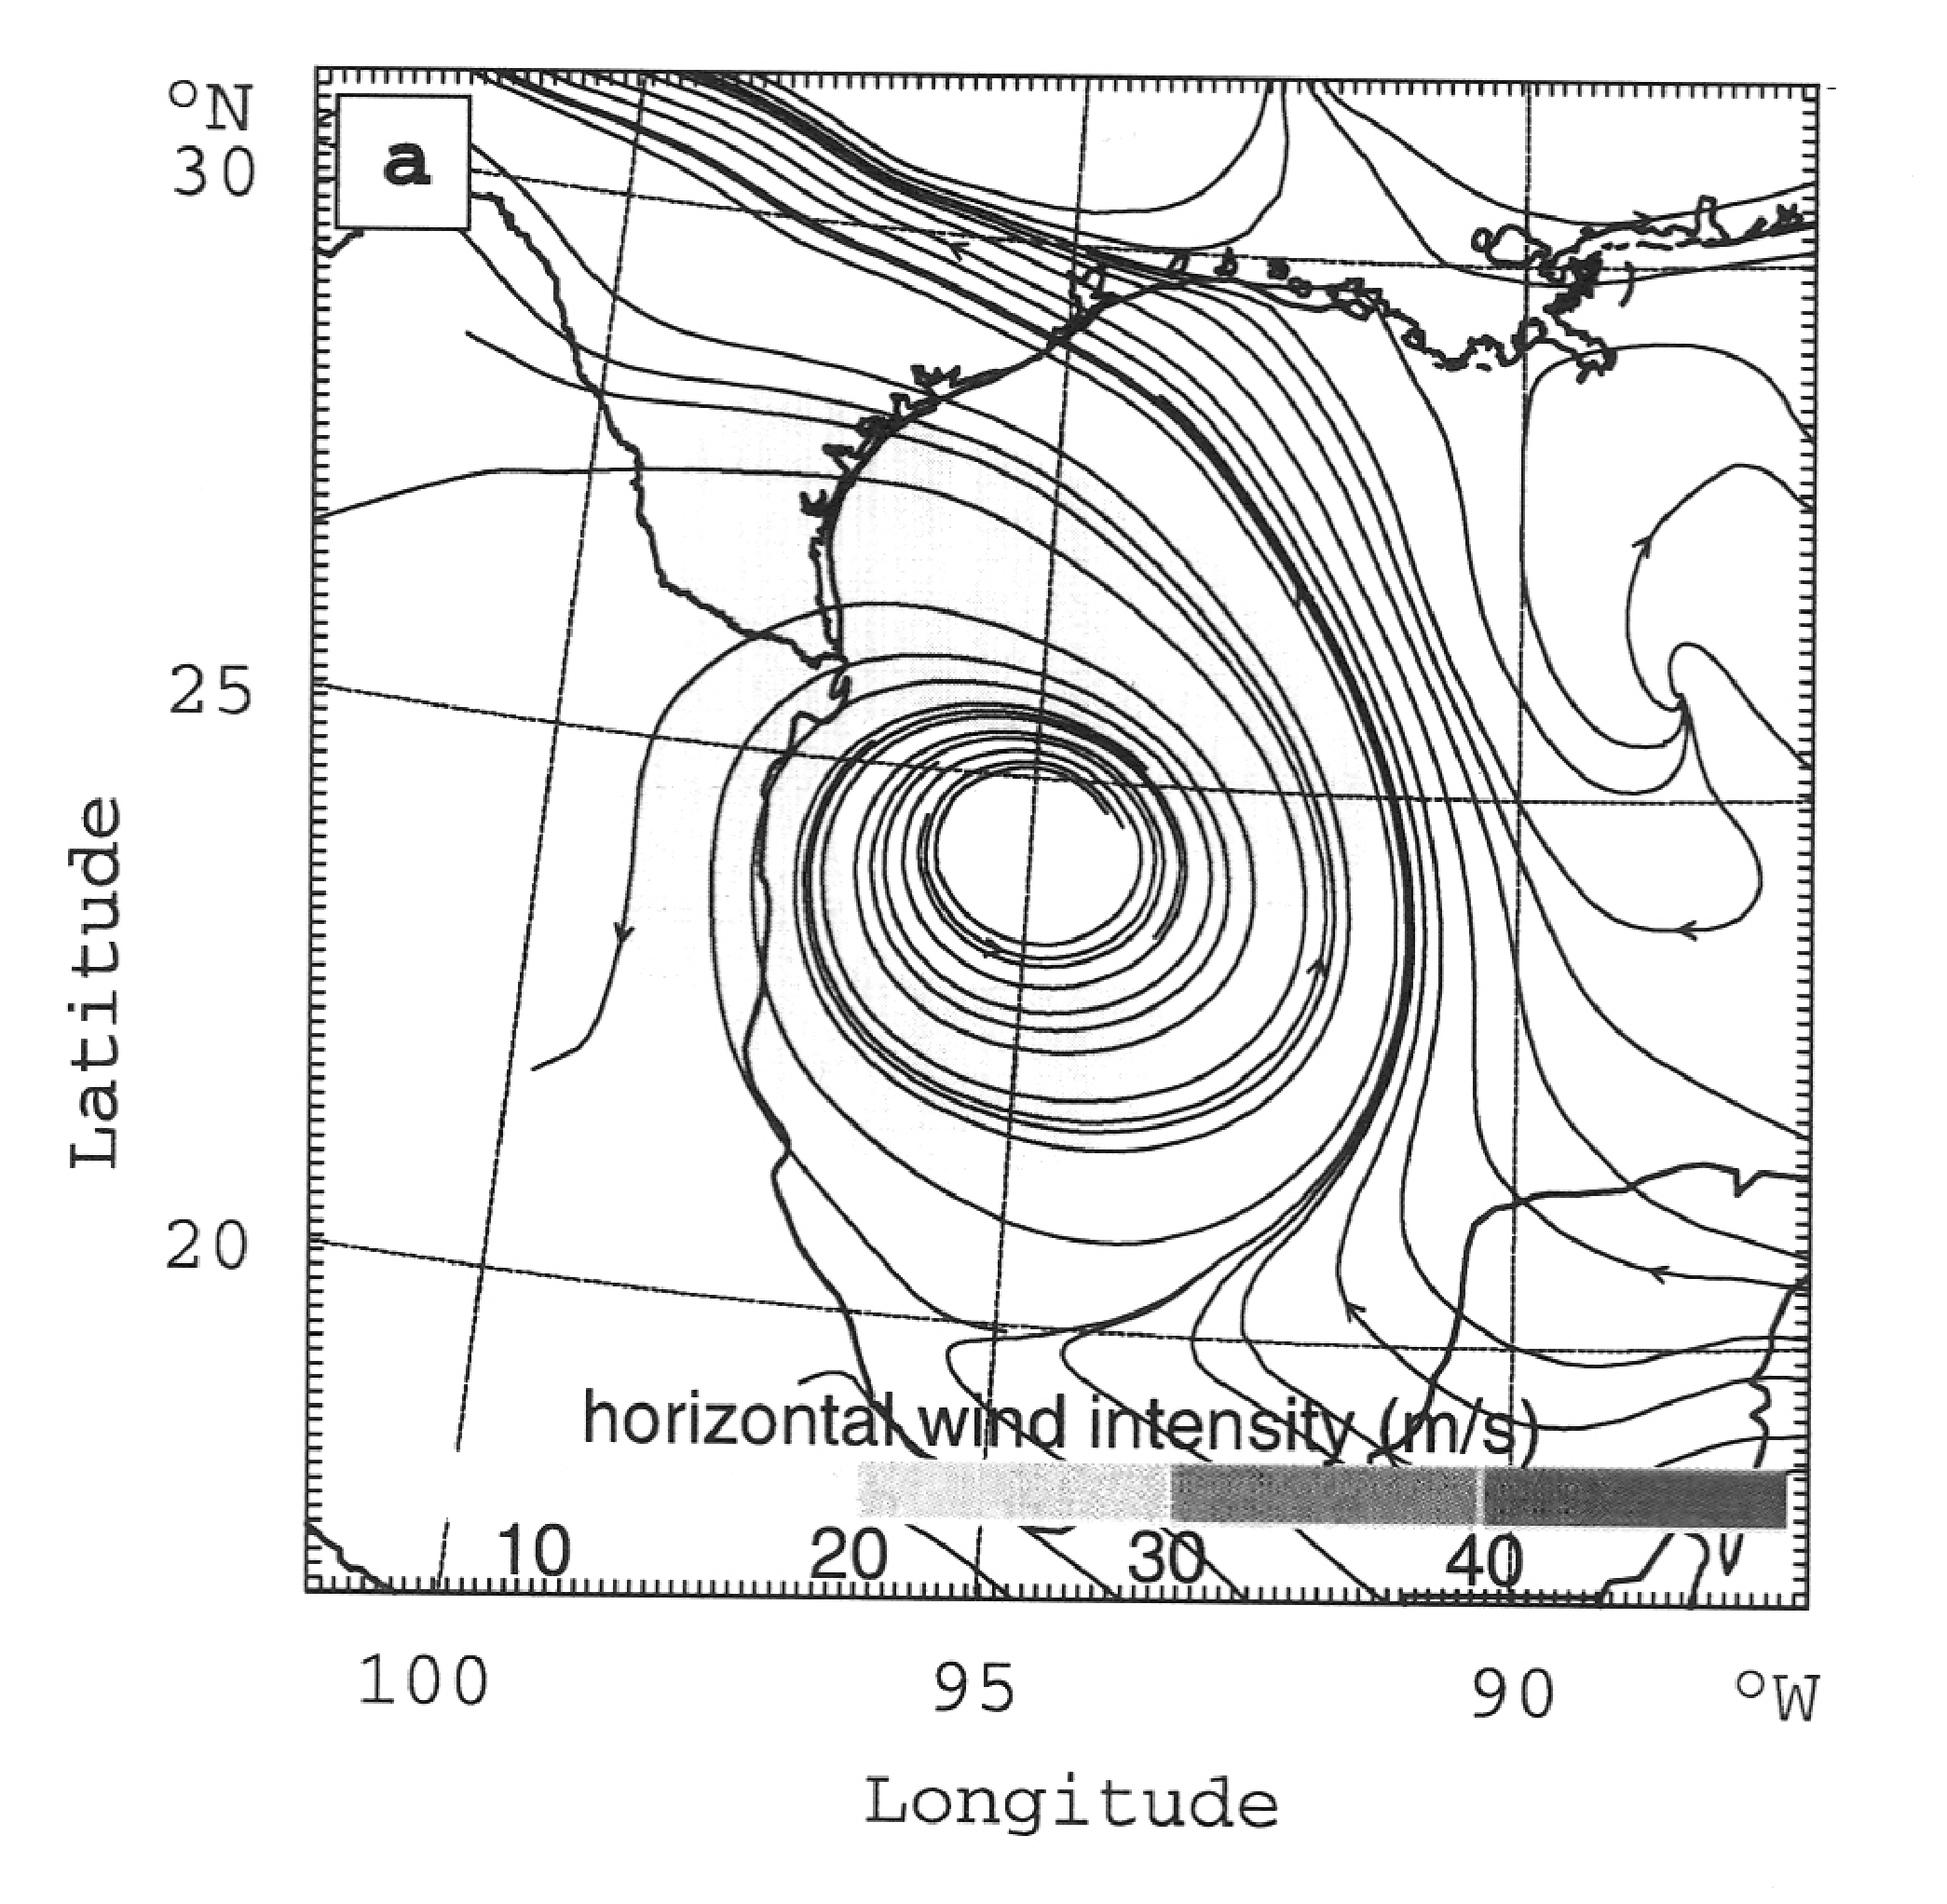
\includegraphics[width=8cm]{\EPSDIR/vortex_ecmwf.eps}&
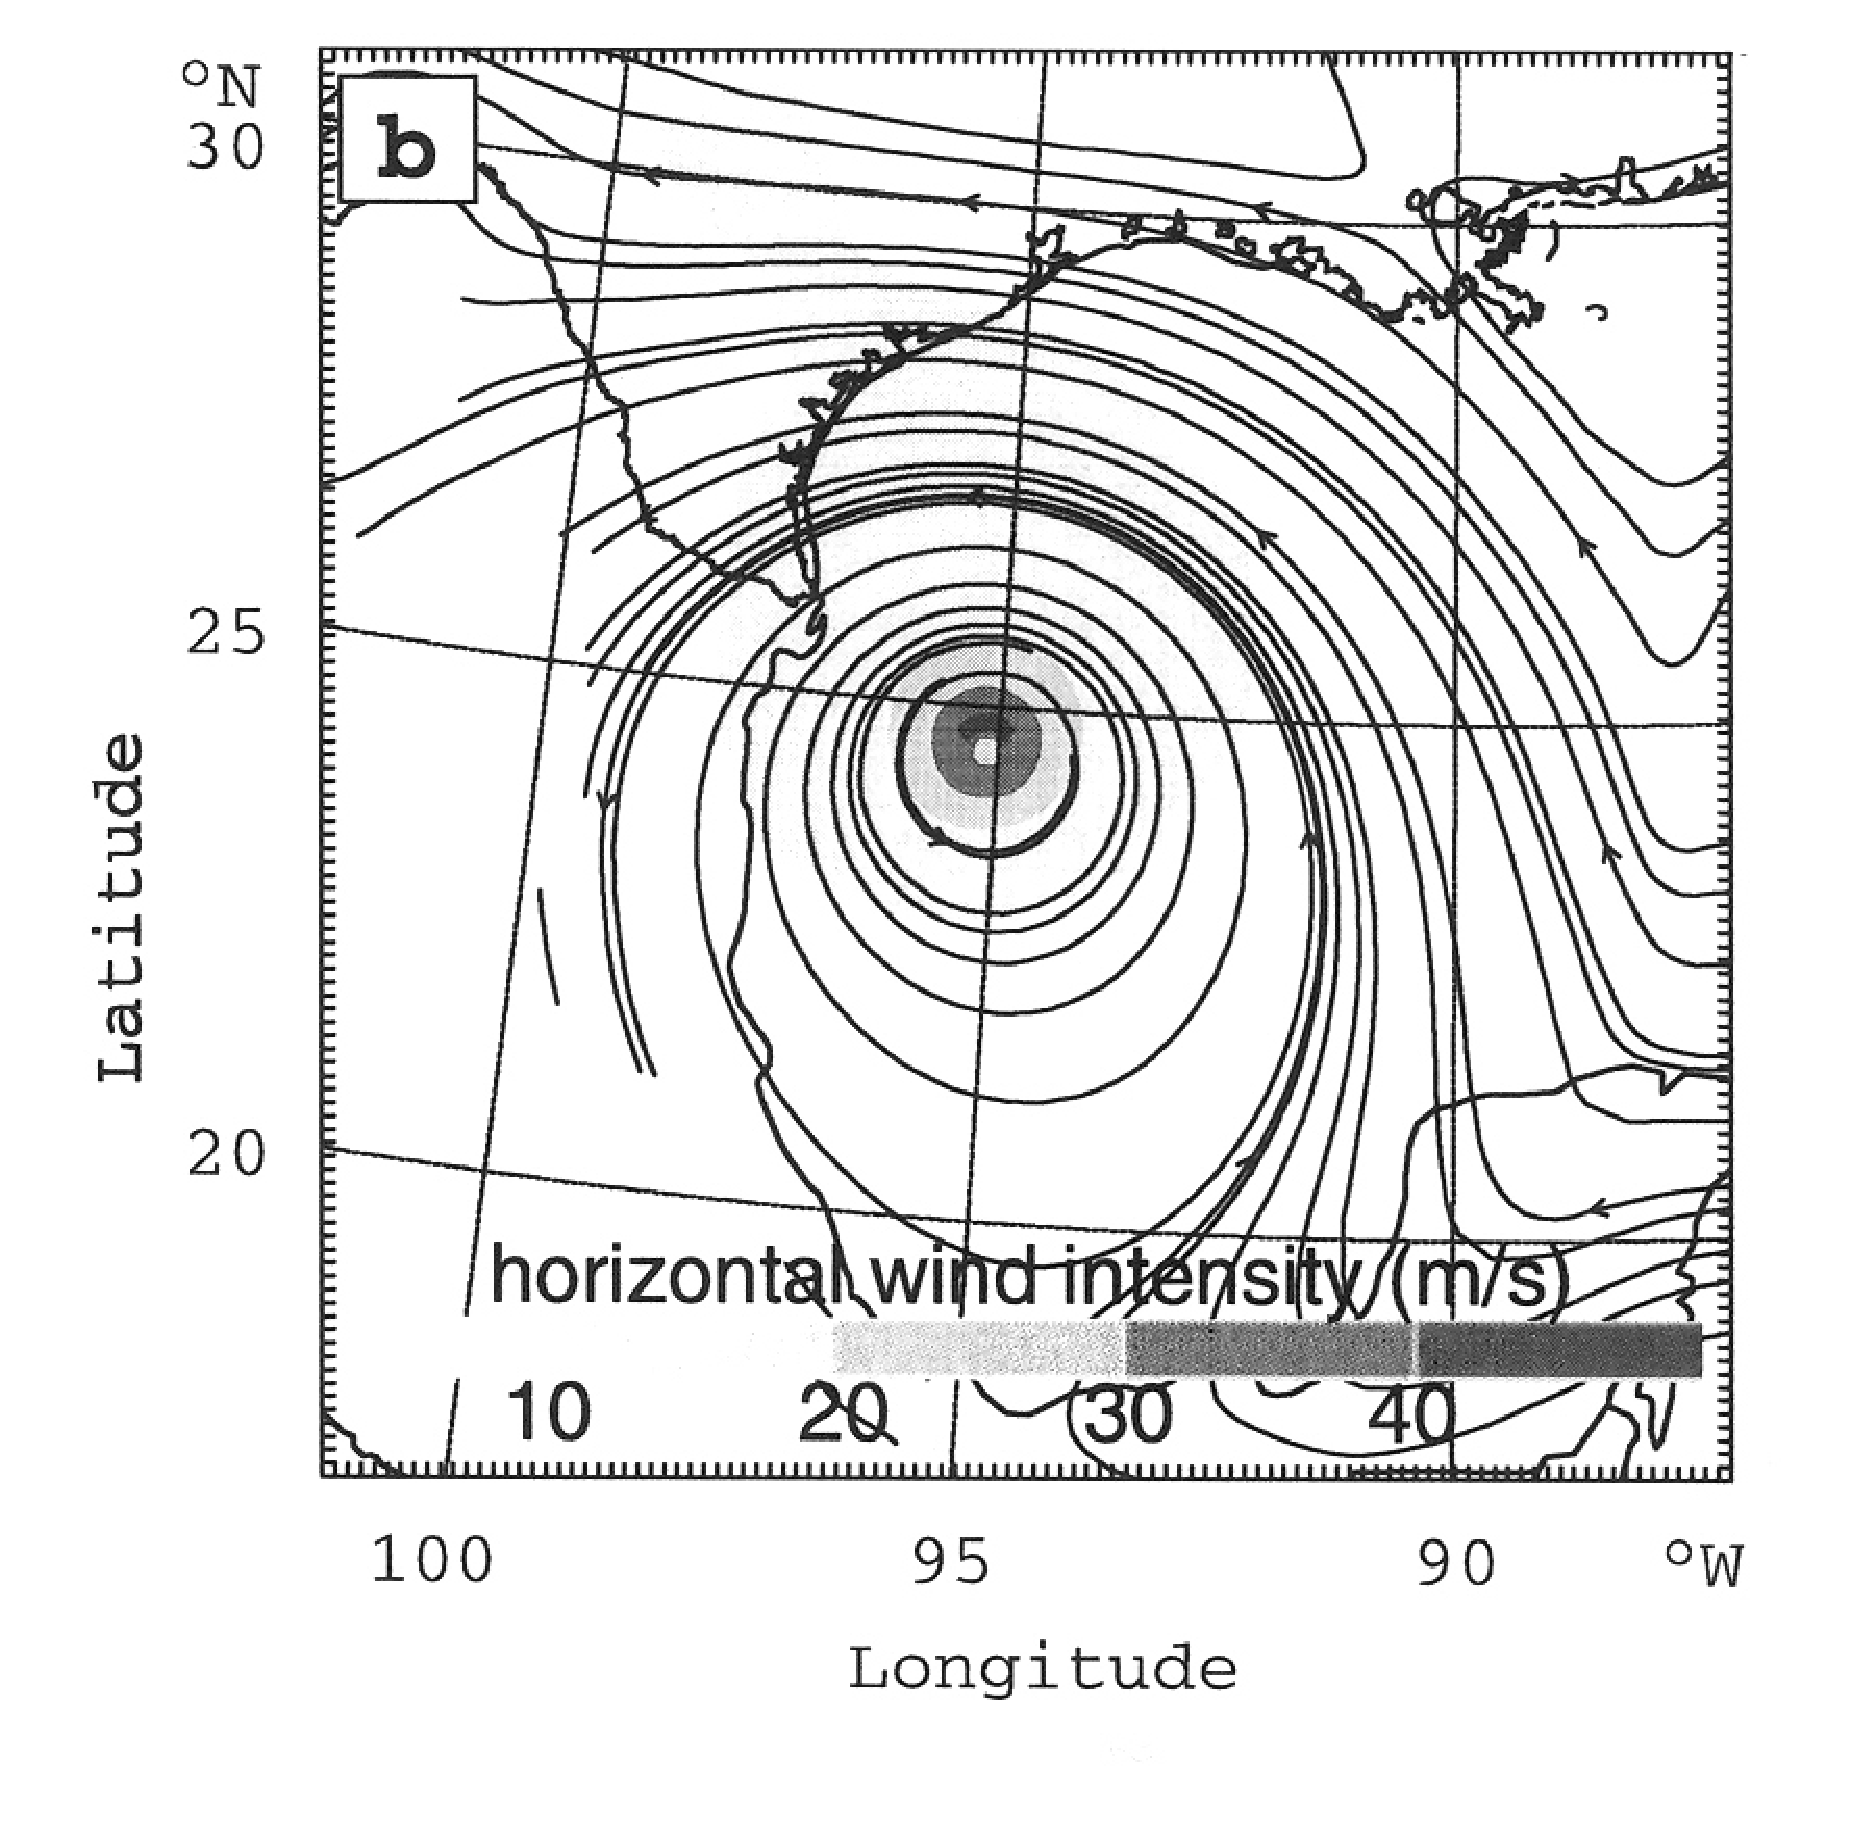
\includegraphics[width=8cm]{\EPSDIR/vortex_radar.eps}\\
\end{tabular}}
\caption{Horizontal streamlines at 850 hPa for Hurricane Bret on 22 August 1999 from (a) the ECMWF global analysis at 00 UTC and (b) the inclusion of the airborne Doppler-derived "specified"}
\label{bogus}
\end{figure}

\section{References}
\noindent
\por
Holland, G. J., 1980:
An analytic model of the wind and pressure profile in hurricanes.
{\it Mon. Weather Rev.}, {\bf 108}, 1212-1218.
\por 
Kurihara, Y., M. A. Bender, and R. J. Ross, 1993:
An initialization scheme of hurricane models by vortex specification.
{\it Mon. Weather Rev.}, {\bf 121}, 2030-2045.
\por
Kurihara, Y., M. A. Bender, R. E. Tuleya, and R. J. Ross, 1995:
Improvements in the GFDL hurricane prediction system.
{\it Mon. Weather Rev.}, {\bf 123}, 2791-2801.
\por 
Nuissier, O., R. F. Rogers, and F. Roux, 2005:
A numerical simulation of Hurricane Bret on 22-23 August 1999
initialized with airborne Doppler radar and dropsonde data.
{\it Quart. J. Roy. Meteor. Soc.}, {\bf 131}, 155-194.
\por
Roux, F. and F. D. Marks Jr, 1996:
Extended Velocity Track Display (EVTD): An improved processing method for 
Doppler radar observations of tropical cyclones.
{\it J. Atmos. Oceanic. Technol.}, {\bf 13}, 875-899.
\por
Roux, F., F. Chane-Ming, A. Lasserre-Bigorry, and O. Nuissier, 2004:
Structure and evolution of intense tropical cyclone Dina near la R\'eunion on 22 
January 2002: GB-EVTD analysis of single Doppler radar observations.
{\it J. Atmos. Oceanic. Technol.}, {\bf 21}, 1501-1518.


